\documentclass[12pt,a4paper]{article}
\usepackage[utf8]{inputenc}
\usepackage[russian]{babel}
\usepackage{amsmath}
\usepackage{amsfonts}
\usepackage{amssymb}
\usepackage{makeidx}
\usepackage[left=3cm, right=3cm, top=1cm, bottom=2cm]{geometry}
\usepackage{graphicx}

\begin{document}

\newcommand{\parw}[2]{\dfrac{\partial #1}{\partial #2}}
\newcommand{\pl}{p_{\lambda}}
\newcommand{\pa}{p_{a}}
\newcommand{\pgm}{p_{m, \sigma^2}}
\newcommand{\pma}{p_{M, a}}
\newcommand{\xseqn}{x_1, \ldots, x_n}
\renewcommand{\le}{\leqslant}


\binoppenalty=10000
\relpenalty=10000
\newcommand*{\hm}[1]{#1\nobreak\discretionary{}%
{\hbox{$\mathsurround=0pt #1$}}{}}

\begin{center}
\textbf{Домашняя работа 1. Отчет.}
\end{center}

\section{Постановка задачи:}

Дано дифференциальное уравнение

$$
\left\{
\begin{array}{lcl}
x' = x + y\\
y' = (\alpha - 1) y + (\alpha - 2) x - x^3 - x^2 y,\\
\end{array}
\right.
$$

где
$
\alpha = \{-1.1, 0.2, 4.7\}
$

Необходимо:
\begin{enumerate}
\item Найти особые точки,
\item Определить типы особых точек,
\item Нарисовать орбиты в окрестностях особых точек,
\item При наличии периодических решений, численно найти их периоды. Оценить погрешность.
\end{enumerate}

\bigskip

\section{Метод решения:}

\begin{enumerate}
\item Особые точки:

$$
\left\{
\begin{array}{lcl}
0 = x + y\\
0 = (\alpha - 1) y + (\alpha - 2) x - x^3 - x^2 y,\\
\end{array}
\right.
$$

$$
\left\{
\begin{array}{lcl}
x = - y\\
0 = - (\alpha - 1) x + (\alpha - 2) x - x^3 + x^3,\\
\end{array}
\right.
$$

$$
\left\{
\begin{array}{lcl}
x = -y\\
x = 0\\
\end{array}
\right.
$$

Отсюда получаем, что $(0, 0)$ --- особая точка.

\item Тип особой точки

Продифференцировав правые части уравнений и подставив координаты особой точки, имеем следующую матрицу:

$$\begin{pmatrix}
1 & 1\\
\alpha - 2 & \alpha - 1\\
\end{pmatrix}$$

Характеристическое уравнение:

$$
\lambda^2 - \alpha \lambda + 1 = 0
$$

$$
\lambda_{1, 2} = \frac{\alpha \pm \sqrt{\alpha^2 - 4}}{2}
$$

Тогда для данных значений $\alpha$ имеем следующие собственные значения:

\begin{enumerate}
\item $\alpha = 1.1$

$$\lambda_{1, 2} = \frac{1.1 \pm \sqrt{2.79} i}{2}$$

Тип особой точки --- неустойчивый фокус

\item $\alpha = 0.2$

$$\lambda_{1, 2} = \frac{0.2 \pm \sqrt{3.96} i}{2}$$

Тип особой точки --- неустойчивый фокус

\item $\alpha = 4.7$

$$
\lambda_1 = 4.47
$$

$$
\lambda_2 = 0.22
$$

Тип особой точки --- неустойчивый узел
\end{enumerate}
\end{enumerate}


\textbf{Итерационный алгоритм поиска периода:}

\begin{enumerate}
\item Взять начальное приближение $(x_0, y_0)$, выбрать случайный луч $l$;
\item На $n$-ом шаге построить $(x_n, y_n)$ по формулам метода Рунге-Кутта двумя способами: с шагом $\tau$ и $0.5 \cdot \tau$. Обновить оценку погрешности;
\item Если расстояние до $(x_n, y_n)$ велико, то считаем, что траектория уходит на бесконечность;
\item Если расстояние до $(x_n, y_n)$ мало по сравнению с текущей оценкой погрешности, то считаем, что траектория стремится к особой точке;
\item Если отрезок $(\{x_{n-1}, y_{n - 1}\}, \{x_n, y_n\})$ пересекает луч $l$, то сравнить значения предыдущей и текущей их точки пересечения. Если расстояние мало по сравнению с оценкой текущей погрешности, то считаем, что период найден;
\item Перейти к шагу 2.
\end{enumerate}

\section{Численные результаты:}

\begin{tabular}{|c|c|c|c|}
\hline 
д & $\tau$ & $T$ & error \\ 
\hline 
-1.1 & 1e-1 & --- & --- \\ 
\hline 
-1.1 & 1e-2 & --- & --- \\ 
\hline 
-1.1 & 1e-3 & --- & --- \\ 
\hline 
-1.1 & 1e-4 & --- & --- \\ 
\hline 
0.2 & 1e-1 & 6.30000 & 9e-5 \\ 
\hline 
0.2 & 1e-2 & 6.30000 & 6e-8 \\ 
\hline 
0.2 & 1e-3 & 6.29900 & 2e-12 \\ 
\hline 
0.2 & 1e-4 & 6.29890 & 1e-13 \\ 
\hline 
4.7 & 1e-1 & 8.80000 & 7e-1 \\ 
\hline 
4.7 & 1e-2 & 11.19000 & 3e-4 \\ 
\hline 
4.7 & 1e-3 & 11.18400 & 2e-7 \\ 
\hline 
4.7 & 1e-4 & 11.18450 & 9e-12 \\ 
\hline 
\end{tabular} 

\subsection{д = $-1.1$}

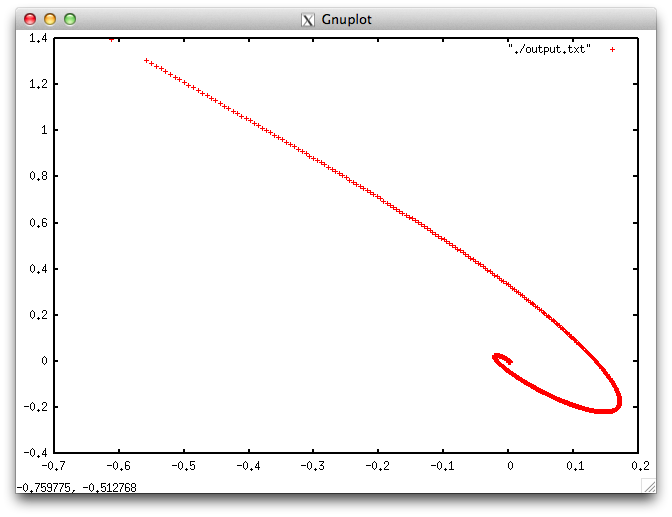
\includegraphics[scale=0.5]{first}

\subsection{д = $0.2$}

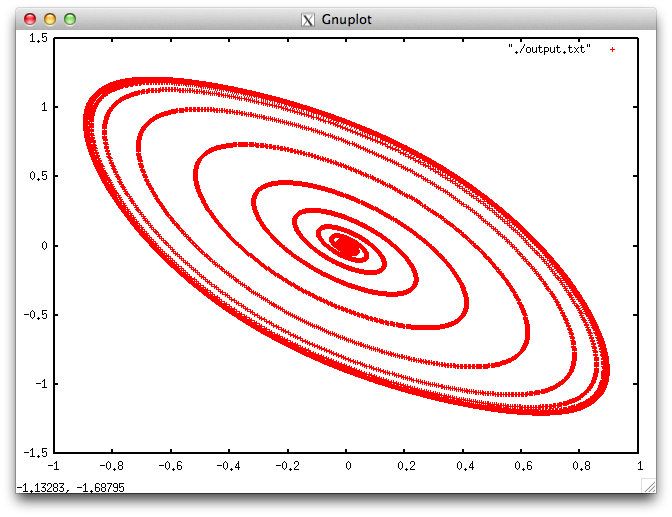
\includegraphics[scale=0.5]{second}

\subsection{д = $4.7$}

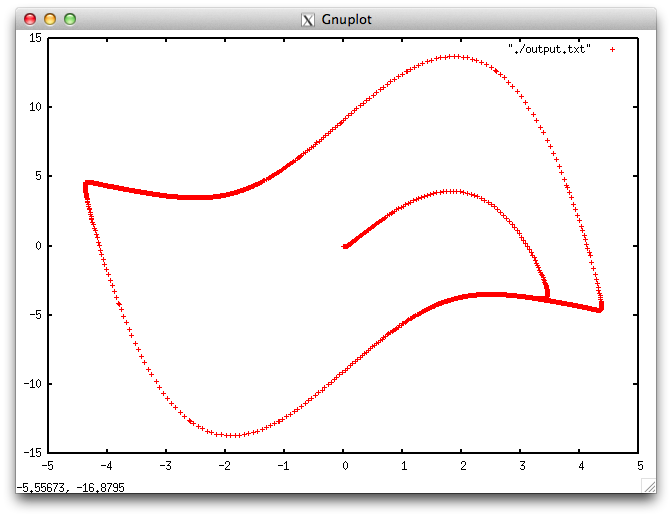
\includegraphics[scale=0.5]{third}

\end{document}


